%%%%%%%%%%%%%%%%%%%%%%%%%%%%%%%%%%%%%%%%%
% Beamer Präsentation
% LaTeX Vorlage
% Version 1.0 (10/11/12)
%
% Diese Vorlage wurde heruntergeladen von:
% http://www.LaTeXTemplates.com
%
% Übersetzt und an eigene Bedürfnisse angepasst von Edgar 'Fast Edi' Hoffmann (08.03.2013)
% Lizenz:
% CC BY-NC-SA 3.0 (http://creativecommons.org/licenses/by-nc-sa/3.0/)
%
%%%%%%%%%%%%%%%%%%%%%%%%%%%%%%%%%%%%%%%%%

%----------------------------------------------------------------------------------------
%	PAKETE UND THEMEN
%----------------------------------------------------------------------------------------

\documentclass{beamer}

\mode<presentation> {

% Die Beamer-Klasse wird mit einer Reihe von Standard Folienthemen,
% mit unterschiedlichen Farben und Folienlayouts. Nachfolgend eine Liste aller verfügbaren Themen.
% Hier kann das jeweils gewünschte Thema unkommentiert werden.

%\usetheme{default}
% \usetheme{AnnArbor}
% \usetheme{Antibes}
% \usetheme{Bergen}
% \usetheme{Berkeley}
% \usetheme{Berlin}
% \usetheme{Boadilla}
% \usetheme{CambridgeUS}
% \usetheme{Copenhagen}
% \usetheme{Darmstadt}
% \usetheme{Dresden}
% \usetheme{Frankfurt}
% \usetheme{Goettingen}
% \usetheme{Hannover}
% \usetheme{Ilmenau}
% \usetheme{JuanLesPins}
% \usetheme{Luebeck}
 \usetheme{Madrid}
% \usetheme{Malmoe}
% \usetheme{Marburg}
% \usetheme{Montpellier}
% \usetheme{PaloAlto}
% \usetheme{Pittsburgh}
% \usetheme{Rochester}
% \usetheme{Singapore}
% \usetheme{Szeged}
% \usetheme{Warsaw}

% Neben verschiedenen Themen kommt die Beamer-Klasse auch mit diversen Farbvarianten
% für jedes Folienthema daher. Hier kann das jeweils gewünschte Farbthema unkommentiert werden.

% \usecolortheme{albatross}
% \usecolortheme{beaver}
% \usecolortheme{beetle}
% \usecolortheme{crane}
\usecolortheme{dolphin}
% \usecolortheme{dove}
% \usecolortheme{fly}
% \usecolortheme{lily}
% \usecolortheme{orchid}
% \usecolortheme{rose}
% \usecolortheme{seagull}
% \usecolortheme{seahorse}
% \usecolortheme{whale}
% \usecolortheme{wolverine}

%----------------------------------------------------------------------------------------
%	DEFINITION BENUTZERDEFINIERTER FARBEN (RGB)
%----------------------------------------------------------------------------------------
\definecolor{dunkelgrau}{rgb}{0.8,0.8,0.8}
\definecolor{hellgrau}{rgb}{0.95,0.95,0.95}
\definecolor{hellblau}{rgb}{0.8,0.85,1}
\definecolor{dunkelblau}{rgb}{0,0,0.9}

% \setbeamertemplate{footline}				% Zum Entfernen der Fusszeile auf allen Folien kann diese Zeile unkommentiert werden
\setbeamertemplate{footline}[frame number]		% Zum Ersetzen der Fußzeile mit einem einfachen Folienzähler kann diese Zeile auskommentiert werden

\setbeamertemplate{navigation symbols}{}		% Zum Anzeigen der Navigationssymbole am unteren Rand aller Folien kann diese Zeile auskommentiert werden
}

\setbeamertemplate{background canvas} [vertical shading][top=hellblau, bottom=white] 

% \usepackage{pgfpages}				% Zum Erstellen vernünftiger Ausdrucke/Handouts diese Zeile(n) unkommentieren
% \pgfpagesuselayout{resize to}[a4paper,border shrink=5mm,landscape]	% Einseitiger Ausdruck auf A4
% \pgfpagesuselayout{2 on 1}[a4paper,border shrink=5mm]			% Druckt 2 Folien auf 1 Seite A4
% \pgfpagesuselayout{4 on 1}[a4paper,border shrink=5mm,landscape]		% Druckt 4 Folien auf 1 Seite A4
% \pgfpagesuselayout{8 on 1}[a4paper,border shrink=5mm]			% Druckt 8 Folien auf 1 Seite A4
% \pgfpagesuselayout{16 on 1}[a4paper,border shrink=5mm,landscape]		% Druckt 16 Folien auf 1 Seite A4

% \setbeameroption{show notes on second screen=right}	% Zum Anzeigen von Notizen auf dem 2. Schirm.  Mit <location> = left, right, bottom oder top
									% Benötigt das Paket pgfpages!

%\beamerdefaultoverlayspecification{<+->}		% Aufzählungen immer schrittweise zeigen

% \setbeamercovered{transparent}			% Sorgt dafür, daß versteckte Textteile nicht unsichtbar, sondern mit wenig Kontast dargestellt werden

\setbeamerfont{frametitle}{family=\sffamily,series=\bfseries,size={\fontsize{18.00}{20.00}}}	% Setzen der Schriftart und -größe für die Überschriften
\setbeamerfont{footline}{family=\sffamily,series=\bfseries,size={\fontsize{6.00}{7.00}}}		% Setzen der Schriftart und -größe für die Fusszeile

\usepackage[ngerman]{babel}				% für Deutsch
%\usepackage{ngerman}
%\usepackage[english]{babel}				% für Englisch
%\usepackage[latin1]{inputenc}
\usepackage[utf8]{inputenc}
\usepackage{graphicx}					% Erlaubt das Einbinden von Grafiken/Bildern
\usepackage{eurosym}					% Erlaubt das Anzeigen des Eurosymbols
\usepackage{xcolor}					% Erlaubt den Einsatz benutzerdefinierter Farben
								% Weitere Einsatzmöglichkeiten:
								% \textcolor{Farbe}{Text} entspricht Befehlen, wie \textbf{}
								% \pagecolor{Name}, \pagecolor{model}{specification} setzt die Hintergrundfarbe der Seite
								% \colorbox{Name}{Text}, \colorbox{model}{specification}{Text} hinterlegt den Text mit der Farbe
								% \fcolorbox{Name}{Text}, \fcolorbox{model}{specification}{Text} umrandet den Text mit der Farbe
								% vordefinierte Farben: black, white, red, green, blue, cyan, magenta, yellow

\usepackage{colortbl}					% Erlaubt das Verwenden benutzerdefinierter Farben in Tabellen
								% \cellcolor{farbe}, \rowcolor{farbe} oder \columncolor{farbe}

\usepackage{url}						% Erlaubt das Verwenden von URLs ohne umständliche Maskierung
\urlstyle{tt}							% Durch Verwendung von \urlstyle{tt} kann zusätzlich die Schriftart auf Typewriter gestellt werden
\urldef{\fsog}{\url}{http://www.FreieSoftwareOG.org}	% Häufig vorkommende URLs können in einem Makro hinterlegt werden.

\usepackage{booktabs}					% Erlaubt den Einsatz von \toprule, \midrule und \bottomrule innerhalb von Tabellen

% \usepackage{fontspec}					% Erlaubt das Anpassen von Schriftarten. Z.B. auch um eigene Fonts zu verwenden. MUSS MIT XELATEX KOMPILIERT WERDEN!!
% \defaultfontfeatures{Mapping=tex-text}
% \setmainfont{Yanone Kaffeesatz}			% (Haupt-)Schriftart der Präsentation

% Will man ein globales Hintergrundbild verwenden, muss dies in der Preamble definiert werden
% Hier verwende ich das der FSOG
%\usebackgroundtemplate%
%{
%  
\includegraphics[width=\paperwidth,height=\paperheight]{../gemeinsam/Praesentationshintergrund}%
%}

\usepackage{pgf}  
\logo{\pgfputat{\pgfxy(-1.2,-0.2)}{\pgfbox[center,base]{
\includegraphics[width=2.6cm]{../gemeinsam/fsog.png}}}}  

%\logo{
\includegraphics[width=3cm]{../gemeinsam/fsog.png}}




%----------------------------------------------------------------------------------------
% DEFINITION DER TITELFOLIE
%----------------------------------------------------------------------------------------

\title[FreieSoftwareOG.org - Backup und Recovery]{Backup und Recovery} % Der Kurztitel (in eckiger Klammer) erscheint im unteren Bereich aller Folien, der Haupttitel (in geschweifter Klammer) erscheint nur auf der Titelfolie

\author{Edgar 'Fast Edi' Hoffmann}    % Name des Vortragenden
\institute[FSOG]          % Die Institution. Erscheint am unteren Rand aller Folien, zum Platz sparen möglichst eine Abkürzung
{
Community FreieSoftwareOG \\      % Die Institution. Erscheint auf der Titelfolie
\medskip
\textit{kontakt@freiesoftwareog.org}    % Die Mailadresse. Erscheint auf der Titelfolie
}
\date{\today}         % Das Datum des Vortrags (hier: aktuelles Datum)

%----------------------------------------------------------------------------------------
% ANFANG DES DOKUMENTES / DER PRÄSENTATION
%----------------------------------------------------------------------------------------

\begin{document}

\begin{frame}     % Der Zusatz [plain] sorgt dafür, daß keine Seitenzahl/Fusszeile verwendet wird
  \titlepage      % Ausgabe der Titelfolie als erste Folie
\end{frame}

%------------------------------------------------------------------------------------------
% AB HIER BEGINNT DIE EIGENTLICHE PRÄSENTATION
%------------------------------------------------------------------------------------------

\begin{frame}
  \frametitle{Backup und Recovery - Begriffserklärung}
  \pause
  Unter Backup versteht man das teilweise oder gesamte Kopieren der in einem Computersystem vorhandenen Daten auf ein alternatives (häufig transportables) Speichermedium.\\ \pause
  Zur wiederherstellbaren vollständigen Datensicherung ist die Fixierung aller Werte bzw. Daten notwendig.\\ \pause
  Die auf dem Speichermedium gesicherten Daten werden als Sicherungskopie, bzw. “Backup” bezeichnet.\\ \pause
  Das Ziel ist, den Datenverlust bei Systemausfällen zu begrenzen, bzw. ganz zu vermeiden.\\ \pause
  Die Wiederherstellung einer Sicherungskopie bezeichnet man als Datenrücksicherung, Restore oder Recovery.
\end{frame}

\begin{frame}
  \frametitle{Warum Backups?}
  \pause
  Neben dem einleuchtenden Grund, Backups zu machen um Datenverlusten vorzubeugen, gibt es auch andere, z.B. gesetzliche Grundlagen:\\ \pause
  \begin{itemize}
    \item Basel II: Backup wirkt sich auf die Kreditwürdigkeite eines Unternehmens aus
    \item ISO/TS 16949: Pflicht!
    \item Ordnungsgemäße, nachvollziehbare, revisionssichere Buchführung (lt. HGB)
  \end{itemize}
\end{frame}

\begin{frame}
  \frametitle{Ursachen von Datenverlusten}
  \pause
  \begin{itemize}
    \item Menschliches Versagen...\\(Hoppla, Verzeichnis gelöscht, "rm -rf /")
    \item Technisches Versagen\\(z.B. Festplattendefekt, Überspannung, etc.)
    \item Umweltgefahren
    \begin{itemize}
      \item Blitz/Sturm/Hagel
      \item Feuer/Löschwasser
      \item Erdbeben
    \end{itemize}
    \item Vandalismus
    \item Diebstahl
  \end{itemize}
\end{frame}

\begin{frame}
  \frametitle{Fragenkatalog}
  \pause
  \begin{itemize}
    \item Wie lange darf ein Computersystem ausfallen bis es wieder läuft?
    \item Auf wieviele, bzw. welche Daten kann ich verzichten?
    \item Was sind die Kosten dieses System, bzw. die Daten wiederherzustellen?
  \end{itemize}
\end{frame}

\begin{frame}

% Hier können Notizen für den Vortragenden auf einem 2. Schirm angezeigt werden. Benötigt die Definition:
% \setbeameroption{show notes on second screen=<location>}
% Mit <location> = left, right, bottom oder top

% \note[item]{Notiz 1}
% \note[item]{Notiz 2}

  \frametitle{Grundlagen}
  \pause
  \begin{itemize}
    \item Die Sicherung sollte immer an einem anderen Ort aufbewart werden als die Originaldaten
    \item Je nach "Wert" der Daten ist es mitunter ratsam, von der Sicherung nochmals eine Kopie anzufertigen. Möglichst auf einem anderen Medium
  \end{itemize}
\end{frame}

\begin{frame}
% \note[item]{Notiz 1}
% \note[item]{Notiz 2}
  \frametitle{Grundlagen}
  \pause
  Der einzig sichere Beweis einer erfolgreichen Datensicherung ist der Nachweis, daß die gesicherten Daten auch vollständig und innerhalb eines angemessenen Zeitraums wiederhergestellt werden können.\\ \pause
  Aus diesem Grund müssen unbedingt in regelmäßigen Abständen Rücksicherungstests erfolgen.\\ \pause
  Wer hat schon jemals ein “Bare-Metal-Recovery” versucht?  \pause
  \begin{alertblock}{Merke:}
    {\bf Es kümmert niemanden, wenn du Backups erstellst.}\\(Nur wenn du Wiederherstellen kannst bist du der King!).
  \end{alertblock}
\end{frame}

\begin{frame}
  \frametitle{Grundlagen}
  Bei der Datensicherung ist es sehr wichtig, eine gute Dokumentation zu führen, da von ihr der Erfolg und die Geschwindigkeit der Datensicherung sowie der Wiederherstellung abhängen können.
  Die Dokumentation sollte umfassen:
  \pause
  \begin{itemize}
    \item Ablauf der Datensicherung
    \item Aufbau der Archivierung
    \item zu treffende (Sofort-)Maßnahmen
    \item Kompetenzen (der Mitarbeiter und Dienstleister)
    \item Prioritäten für besonders zeitkritische Daten und Systeme
  \end{itemize}
  \pause
Für eine bessere Übersichtlichkeit ist die Dokumentation für Sicherung und Wiederherstellung jeweils getrennt in einem Sicherungs- bzw. Wiederherstellungsplan festzulegen.
\end{frame}

\begin{frame}
  % \note[item]{Notiz 1}
  \frametitle{Backup-Methoden:\\Vollständige Sicherung}
  \pause
  Eine vollständige Datensicherung bezeichnet die Sicherung aller Daten, unabhängig vom Datum ihrer letzten Sicherung.\\
  \pause
  \vspace{10mm}
  \begin{center}
    
\includegraphics[width=0.9\linewidth]{Bilder/Vollbackup}
  \end{center}
\end{frame}

\begin{frame}
  \frametitle{Backup-Methoden:\\Inkrementelle Sicherung}
  \pause
  Bei der inkrementellen Sicherung werden immer nur die Dateien gespeichert, die seit der letzten inkrementellen Sicherung oder (bei der ersten inkrementellen Sicherung) seit der letzten Komplettsicherung geändert wurden oder neu hinzugekommen sind. Es wird also immer auf der letzten inkrementellen Sicherung aufgesetzt. Die Vorteile sind eine geringere zu sichernde Datenmenge und schnellere Datensicherung. Der Nachteil ist ein relativ großer Aufwand bei der Wiederherstellung von Daten, da mehrere Sicherungen hintereinander überspielt werden müssen.\\
  \pause
  \vspace{10mm}
  \begin{center}
    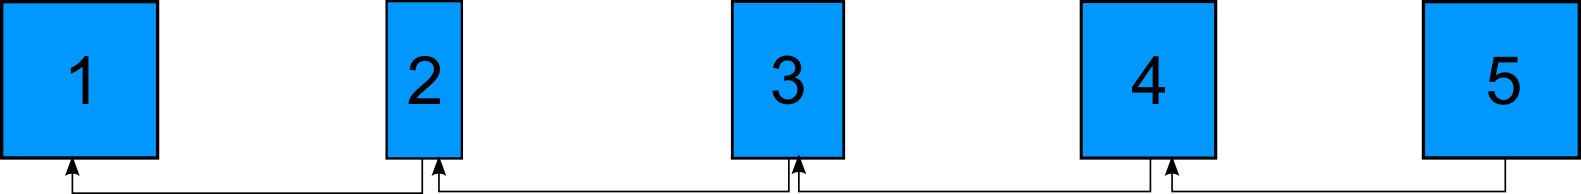
\includegraphics[width=0.9\linewidth]{Bilder/InkrementellesBackup}
  \end{center}
\end{frame}

\begin{frame}
  \frametitle{Backup-Methoden:\\Differenzielle Sicherung}
  \pause
  Bei der sogenannten differenziellen Sicherung werden alle Daten, die seit der letzten Komplettsicherung geändert wurden oder neu hinzugekommen sind, gespeichert. Es wird also immer wieder auf der letzten Komplettsicherung aufgesetzt, wobei gegenüber einer neuen Vollsicherung Speicherplatz und Zeit gespart werden kann.
  \pause
  \vspace{10mm}
  \begin{center}
    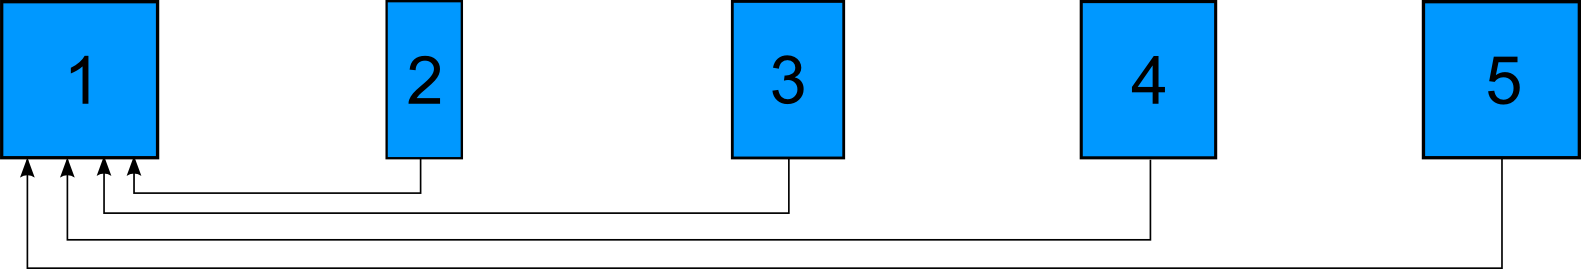
\includegraphics[width=0.9\linewidth]{Bilder/DifferenziellesBackup}
  \end{center}
\end{frame}

\begin{frame}
  \frametitle{Backup-Methoden:\\Fortschreitende inkrementelle Sicherung}
  \pause
  \begin{itemize}
    \item Es werden ausschließlich und beliebig oft nur veränderte oder neu hinzugekommene Dateien gesichert
    \item Eine vollständige Sicherung wird nur implizit im Rahmen der Einrichtung des Sicherungsbetriebs gemacht
    \item Beim Wiederherstellen bietet das Datensicherungsprogramm virtuell zusammengesetzte Vollsicherungen zur Auswahl an
    \item Das verbindet die Vorteile der Vollsicherung\\(einfache Handhabung)\\mit inkrementeller Sicherung\\(kleine Datenmengen)
    \item Nachteil: Komplexität des Werkzeugs\\(Datenbankbasiertes Datensicherungsprogramm)
    \item Beispiel: Die Wiederherstellungskonsole in Windows
  \end{itemize}
\end{frame}

\begin{frame}
  \frametitle{Backup-Methoden:\\Großvater - Vater - Sohn}
  \pause
  Eine Großvater-Vater-Sohn Datensicherung, auch Generationenprinzip genannt, ist ein altbekanntes Verfahren zur Datensicherung\\
  \pause
  Dabei wird von dem Datenbestand ständig ein dreifaches Backup verschiedenen Alters (Großvater, Vater, Sohn) von einem Datenträger gemacht\\
  \pause
  Veränderungen und Verluste von Daten können somit rekonstruiert werden\\
  \pause
  Sind die Sohn-Daten beschädigt, werden sie aus den Vater-Daten wieder erzeugt und die Vater-Daten gegebenenfalls aus den Großvater-Daten
\end{frame}

\begin{frame}
  \frametitle{Backup-Medien:\\CDs, DVDs und Blu-Rays}
  \pause
  Es gibt verschiedene Studien, welche zusammengenommen nicht sehr hilfreiche Werte nennen:\\
  \pause
  Von wenigen Monaten bis zu mehreren Jahren...\\
  \pause
  Die Qualität der Sicherung hängt vom Brenner, Rohling und lesendem Laufwerk ab\\
  \pause
  Wichtig bei der Verwendung dieser Medien sind regelmäßige Tests bzw. Umkopieren
\end{frame}

\begin{frame}
  \frametitle{Backup-Medien:\\USB-Sticks, -Festplatten, Bänder}
  \pause
  \begin{itemize}
    \item USB-Sticks
      \begin{itemize}
        \item Relativ sicher
        \item Haltbarkeit durch die Natur des Mediums begrenzt
        \item Bei Defekt nur sehr eingeschränkte Möglichkeit der Wiederherstellung
      \end{itemize}
    \item USB-Festplatten
      \begin{itemize}
        \item Sehr sicher
      \end{itemize}
    \item (Magnet-) Bänder
      \begin{itemize}
        \item Sehr sicher
        \item Im Privatbereich jedoch nicht verbreitet
      \end{itemize}
  \end{itemize}

\end{frame}

\begin{frame}
  \frametitle{Backup-Medien:\\Die Lagerung}
  \pause
  \begin{itemize}
    \item Die USB-Platte nicht angeschlossen am Rechner lagern
    \item Bänder bei Konstanter Temperatur und trocken lagern (möglichst in einem anderen Brandabschnitt)
    \item Feuerfester Tresor, bzw. überhaupt abgeschlossener Tresor
    \item Externe Sicherheitskopie
      \begin{itemize}
        \item Ein Bankschließfach kostet ca. \euro{30.00} im Jahr
        \item Billiger bei einem Bekannten, und ein Grund auf ein Bier vorbei zu kommen...
      \end{itemize}
  \end{itemize}
\end{frame}

\begin{frame}
  \frametitle{Backup-Medien:\\Geschwindigkeiten}
  \begin{tiny}
  \begin{table}
    \begin{tabular}{l l}
      \toprule        % Zieht eine Linie über der nachfolgenden Tabellenzeile (benötigt Paket "booktabs")
      \textbf{Medium} & \textbf{Geschwindigkeit}\\
      \midrule        % Zieht eine Linie (benötigt Paket "booktabs")
      CD/DVD & ca. 1,5 MB/Sek. bei langsamer, archivtauglicher Geschwindigkeit \\
      \midrule
      Blu-ray & ab 4,5 MB/Sek. (abhängig von Rohling und Brenner) \\
      \midrule
      USB 2 & 60 MB/Sek. (theoretisch) - ~30 MB/Sek. (praktisch) \\
      \midrule
      USB 3 & ab 100 MB/Sek. (abhängig von Gerät und Anbindung) \\
      \midrule
      SATA/SAS & 3 Gbit/Sek. (theoretisch) - ~100 MB/Sek. (praktisch) \\
      \midrule
      Ethernet & 1Gbit/Sek., bzw. 10 Gbit/Sek. (~60MB/Sek. praktisch bei 1Gbit) \\
      \midrule
      Digital Linear Tape (DLT) & ca. 60-120 MB/Sek. \\
      \bottomrule       % Zieht eine Linie unter der vorherigen Tabellenzeile (benötigt Paket "booktabs")
    \end{tabular}
    \caption{Geschwindigkeiten ausgesuchter Medien}
  \end{table}
  \end{tiny}
\end{frame}

\begin{frame}
  \frametitle{Backup-Medien:\\"Lifecycle-Management"}
  \pause
  Wie sieht es aus technischer Sicht mit der Lesbarkeit des gewählten Backup-Mediums aus?\\
  \pause
  Vor 4 Jahren hatte ich in diesem Vortrag noch Zip- und LS120-Laufwerke erwähnt...\\
  \pause
  \begin{alertblock}{Vorschlag:}
      {\bf Neben dem regelmäßigen Umkopieren sollte auch ein Medienwechsel geprüft werden.}\\(Eventuell ist was neues auf dem Vormarsch).
    \end{alertblock}
\end{frame}

\begin{frame}
  \frametitle{Backup-Medien:\\RAID}
  \begin{center}
    Falls es bisher noch niemand erwähnt hat:\\
    \pause
    \vspace{10mm}
    \textcolor{red}{{\Huge RAID ist \underline{kein} Backup!}}
  \end{center}
\end{frame}

\begin{frame}
  \frametitle{Backup im Business-Bereich}
  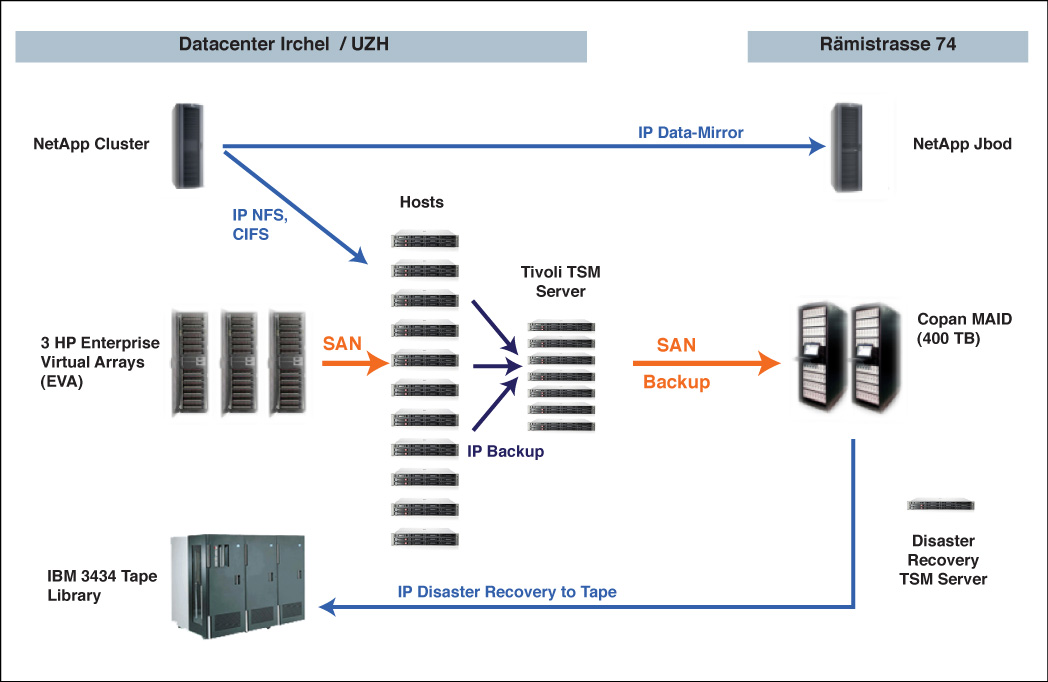
\includegraphics[width=0.9\linewidth]{Bilder/UniZuerichBackup}
  Backup-Schema der Uni Zürich
\end{frame}

\begin{frame}
  \frametitle{Backup im Business-Bereich:\\Online-Spiegelung}
  \pause
  \begin{itemize}
    \item Cluster
    \item SAN über zwei Serverräume
    \item SAN über zwei Rechenzentren
  \end{itemize}
\end{frame}

\begin{frame}
  \frametitle{Backup im Business-Bereich:\\Sicherheit}
  \pause
  Heute ist es kein Problem, den kompletten Datenbestand z.B. der Personalabteilung auf einer Festplatte im Zigarettenschachtelformat unterzubringen.\\
  \pause
  Oder Datenträger mit Sozialversicherungsdaten einer ganzen Stadt werden verloren.\\
  \pause
  \begin{alertblock}{Einzige Möglichkeit, den Verlust einzugrenzen:}
      {\bf Starke Verschlüsselung der gesicherten Daten!}\\(In vielen Firmen sogar Pflicht!).
    \end{alertblock}
\end{frame}

\begin{frame}
  \frametitle{Backup im Business-Bereich:\\Zeitlicher Rahmen (Backup)}
  \pause
  Je nach Volumen kann es lange dauern, Backups zu erstellen.\\
  \pause
  Deshalb arbeitet man im virtuellen Umfeld oder im SAN-Bereich gerne mit sogenannten Snapshots.\\
  \pause
  Dann bleibt einem alle Zeit der Welt um die Daten konsistent abzuziehen.\\
  \pause
  Vorraussetzung hierfür ist genügend primärer Speicher für die Daten die im Backupfenster auflaufen.\\
  \pause
  Denn wenn der Snapshotplatz volläuft, ist der Snapshot unbrauchbar.
\end{frame}

\begin{frame}
  \frametitle{Backup im Business-Bereich:\\Zeitlicher Rahmen (Restore)}
  \pause
  Die Zeit, welche für eine Rücksicherung benötigt, bzw. sogar vorgegeben wird ist genauso wichtig.\\
  \pause
  Theoretische Minimums sind oft nicht realistisch, da bei vielen Dateien Suchzeiten auftreten können.\\
  \pause
  Man wird bei einem File-Server kaum ein Block-Level Backup durchführen.\\
  \pause
  Hinzu kommen noch die Zeiten für die inkrementellen Restores.
\end{frame}

\begin{frame}
  \frametitle{Backup-Software:\\Image-Programme}
  \pause
  \begin{itemize}
    \item Clonezilla
    \item RedoBackup
    \item PING (PartImage is Not Ghost)
  \end{itemize}
\end{frame}

\begin{frame}
  \frametitle{Backup-Software:\\Datei-Backups}
  \pause
  \begin{itemize}
    \item Areca
    \item Cedar-Backup
    \item BackupPC
    \item Bacula
  \end{itemize}
\end{frame}

\begin{frame}
  \frametitle{Backup-Software:\\Die "Cloud"}
  \pause
  Weitere Möglichkeiten der Datensicherung bietet natürlich die immer weiter fortschreitende Cloud-Technologie.\\
  \pause
  Ob man nun Google seine Daten anvertrauen möchte oder nicht, bleibt natürlich jedem selbst überlassen.\\
  \pause
  Clevere Community-Mitglieder haben hier aber ja schon gezeigt, daß man seine Daten auch in einer eigenen Wolke haben kann.
\end{frame}

\begin{frame}
  \frametitle{Backup-Software:\\Die "Cloud"}
  Mögliche Online-Storage-Lösungen:
  \pause
  \begin{itemize}
    \item Google Drive
    \item SkyDrive
    \item Dropbox
    \item OwnCloud
  \end{itemize}
\end{frame}

%------------------------------------------------
% LINKFOLIE
%------------------------------------------------
\begin{frame}[fragile]   % Die "fragile"-Option muss verwendet werden, wenn auf der Folie verbatim verwendet wird
  \frametitle{Links zur Präsentation}
  \begin{verbatim}
    http://www.clonezilla.org
    http://www.redobackup.org
    http://ping.windowsdream.com/
    http://www.areca-backup.org
    http://cedar-backup.sourceforge.net
    http://backuppc.sourceforge.net/
    http://www.bacula.org
  \end{verbatim}
\end{frame}

\begin{frame}
\frametitle{Weitere Informationen bekommen Sie hier:}
  \begin{center}
  \Large{
    \fsog \\      % Makro für das Einfügen der URL (oben definiert)
    und \\
    Kontakt@FreieSoftwareOG.org \\~\\

    oder kommen Sie doch einfach zu unserem regelmäßigen Treffen, \\
    jeden 1. Mittwoch im Monat ab 20:00 Uhr. \\
    (Treffpunkt und Thema laut Webseite)
    }
  \end{center}
  \begin{figure}[ht]
    \centering
    
\includegraphics[width=0.2\textwidth]{../gemeinsam/CC-BY-SA.png}
  \end{figure}  
\end{frame}


\end{document}
